% coding:utf-8

% Ausführen in R: 
% Sweave("C:/Daten/Daniel/studium/git_repo/sem2/stoc/sw06/sw06_4.Rnw",encoding='UTF-8')

\section{Aufgabe 4}

\subsection{a}
\begin{Schunk}
\begin{Sinput}
> ## 20 Werte simulieren
> # p <- seq(from=0,to=1,length.out=20)
> p <- 0.5
> x <- rbinom(20, 50, p)
> ## Grenzen der Intervalle in Matrix speichern
> ## 1. Spalte ist untere Grenze, 2. Spalte obere
> confint.bound <- matrix(0, nrow = 20, ncol = 2)
> contains.truth <- logical(20)
> ## Alle 20 Faelle untersuchen und Grenzen speichern
> for(i in 1:20){
+ test <- binom.test(x=x[i],n=50,p=p,conf.level=0.95) ## Setzen Sie die richtigen Argumente!
+ confint.bound[i,] <- test$conf.int
+ contains.truth[i] <-
+ (p >= confint.bound[i,1]) & (p <= confint.bound[i,2])
+ }
> sum(contains.truth)
\end{Sinput}
\begin{Soutput}
[1] 20
\end{Soutput}
\end{Schunk}

\subsection{b}
\begin{Schunk}
\begin{Sinput}
> ## Relative Haeufigkeiten plotten
> plot(x / 50, 1:20, xlim = c(0, 1), xlab = "Probability",
+ ylab = "Simulation Number")
> ## Vertrauensintervalle als Liniensegemente plotten
> for(i in 1:20){
+ segments(confint.bound[i,1], i, confint.bound[i,2], i)
+ }
> ## Wahrer Wert als vertikale Linie einzeichnen
> abline(v = p)
\end{Sinput}
\end{Schunk}
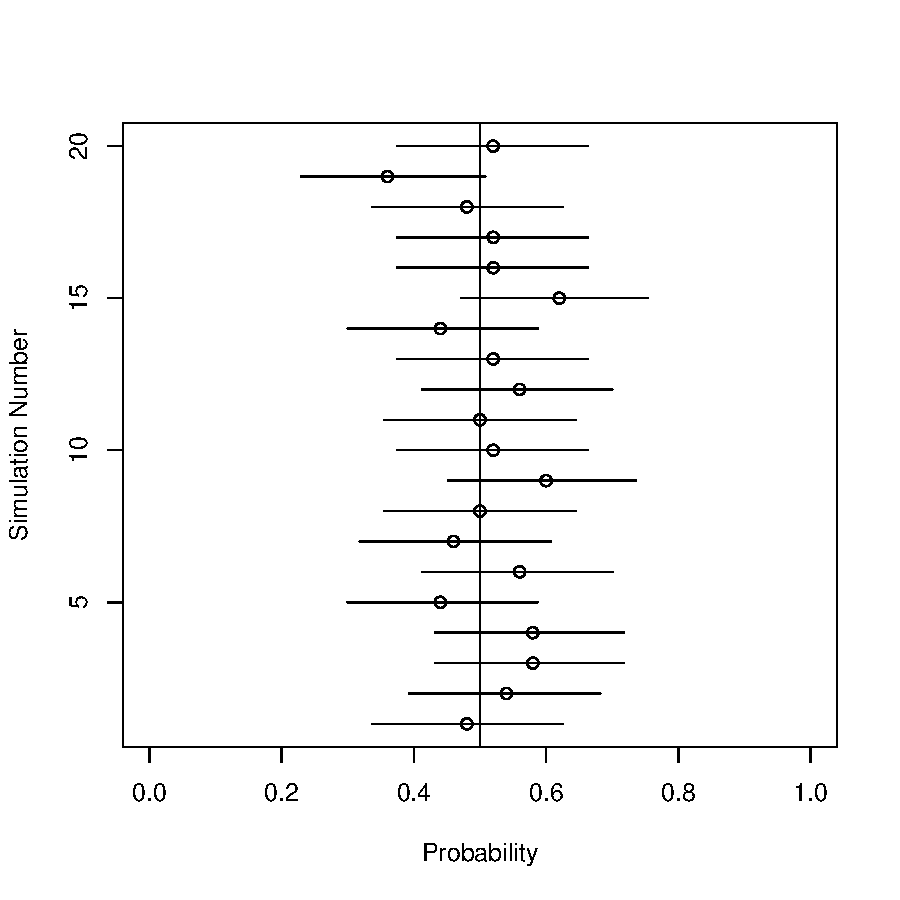
\includegraphics{sw06_4-002}
